\chapter{Epipolar Geometry}
\label{ch:lesson28}

Chapter~\ref{ch:lesson22}'s stereo matching assumed a \emph{rectified} pair, where corresponding points always fall on the same row. In the more general case, stereo cameras may not be rectified. This chapter covers the general two-view relationship between \textbf{any} pair of images of a static scene: a point's match in the other image isn't just \emph{somewhere} --- it's constrained to lie on a particular line. We cover both the calibrated and uncalibrated cases.

\section{The epipolar constraint}

For a point $x_1$ in image 1 and its true match $x_2$ in image 2 (both in homogeneous pixel coordinates), there's a $3\times3$ rank-deficient matrix $F$ --- the \textbf{fundamental matrix} --- such that
\begin{equation}
x_2^\top F x_1 = 0
\end{equation}
for \emph{every} corresponding pair, regardless of scene geometry. $F$ depends only on the two cameras' relative pose and (uncalibrated) intrinsics. Rearranged, $l_2=Fx_1$ is the \textbf{epipolar line} in image 2: the 1D line along which $x_1$'s match is guaranteed to lie. This is exactly the mechanism that made Chapter~\ref{ch:lesson22}'s row-restricted search valid --- rectification is just the special camera arrangement where every epipolar line happens to be horizontal, which collapses the 1D search to a single row.

\subsection*{Why a line? A geometric picture}

Camera 1 knows only the \emph{direction} to a point, not its depth: the true 3D point $X$ could be anywhere along the ray from $C_1$ through $x_1$. But every point on that ray, together with $C_1$ and $C_2$, lies in a single plane --- the \textbf{epipolar plane}. Camera 2 sees this plane edge-on, as a single line: wherever $X$ actually sits along the ray, its projection into image 2 always falls on that one line, the epipolar line, as Figure~\ref{fig:l28-1} illustrates.

\begin{figure}[h]
\centering
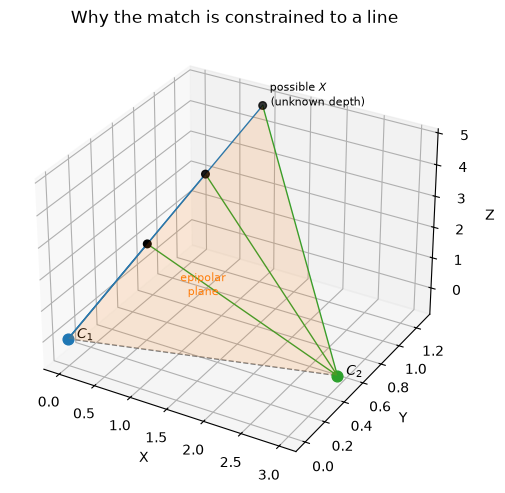
\includegraphics[width=0.55\textwidth]{figures/lesson28_fig01.png}
\caption{Three candidate depths for the same pixel $x_1$, all lying in one epipolar plane; their projections into camera 2 all fall on the same epipolar line.}
\label{fig:l28-1}
\end{figure}

\section{A synthetic two-camera scene}

Build two cameras with known intrinsics $K$ and a known relative rotation/translation, create random 3D points, project them into both cameras (Figure~\ref{fig:l28-2}), and use the resulting correspondences to recover $F$.

\begin{figure}[h]
\centering
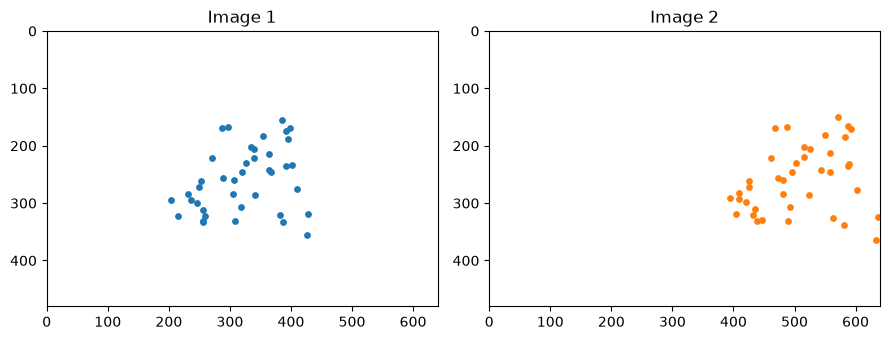
\includegraphics[width=0.9\textwidth]{figures/lesson28_fig02.png}
\caption{40 3D points projected into both cameras.}
\label{fig:l28-2}
\end{figure}

\section{SVD: singular value decomposition}

In Chapter~\ref{ch:lesson23}, we saw that a real symmetric positive-semidefinite matrix $A$ can be written as $A=P\Lambda P^\top$, with $P$ the eigenvectors and $\Lambda$ the (non-negative, diagonal) eigenvalues. The \textbf{singular value decomposition (SVD)} generalizes this: any matrix $A$ --- symmetric or not, square or not --- can be written as $A=U\Sigma V^\top$, with $U,V$ orthogonal (the \textbf{singular vectors}) and $\Sigma$ diagonal and non-negative (the \textbf{singular values}, sorted largest to smallest). Two facts matter here:

\textbf{Solving $Ax=0$ as closely as possible, subject to $\|x\|=1$.} The answer is $V$'s last column --- the right singular vector for the smallest singular value. This is Chapter~\ref{ch:lesson23}'s total-least-squares trick, generalized: $V$'s columns are the eigenvectors of $A^\top A$, sorted by eigenvalue.

\textbf{Enforcing a rank constraint.} Zeroing the smallest singular value(s) and reconstructing gives the closest lower-rank matrix (in a least-squares sense) to the original --- exactly what's needed to force the estimated $F$, which must be exactly rank 2, back onto that constraint after an unconstrained solve drifts off it slightly.

\section{The 8-point algorithm}

Each correspondence gives one linear equation in the 9 unknown entries of $F$ (expanding $x_2^\top F x_1=0$). $F$ is only defined up to scale (like the homography in Chapter~\ref{ch:lesson24}), so it really has just 8 independent unknowns, solvable as a homogeneous least-squares problem via SVD --- the same DLT machinery used for the homography fit. Since $F$ must be exactly rank 2, project the 9-parameter solution back onto the nearest rank-2 matrix using the SVD trick above.

$F$ actually has only 7 true degrees of freedom, since the rank-2 constraint removes one more; a 7-point algorithm exists but is nonlinear, which is why the linear 8-point algorithm (with its separate rank-2 cleanup step) remains popular. Raw pixel coordinates (in the hundreds) also make the linear system badly conditioned, so points are first rescaled to be centered at the origin with average distance $\sqrt2$, solved in normalized coordinates, then the rescaling is undone on the resulting $F$ --- the \textbf{normalized 8-point algorithm} (\citelink{hartley1997}{Hartley, 1997}), the version used here and worth reaching for in practice.

\begin{lstlisting}
_, _, Vt = np.linalg.svd(A)
F = Vt[-1].reshape(3, 3)
U, S, Vt2 = np.linalg.svd(F)   # enforce rank-2 by zeroing the smallest singular value
S[-1] = 0
F = U @ np.diag(S) @ Vt2
\end{lstlisting}

A from-scratch implementation matches \code{cv2.findFundamentalMat(x1, x2, cv2.FM\_8POINT)} to 5 decimal places, and both achieve a mean $|x_2^\top F x_1|$ residual on the order of $10^{-7}$--$10^{-15}$ --- effectively zero. Figure~\ref{fig:l28-3} plots several points' predicted epipolar lines directly, using this recovered $F$.

\begin{figure}[h]
\centering
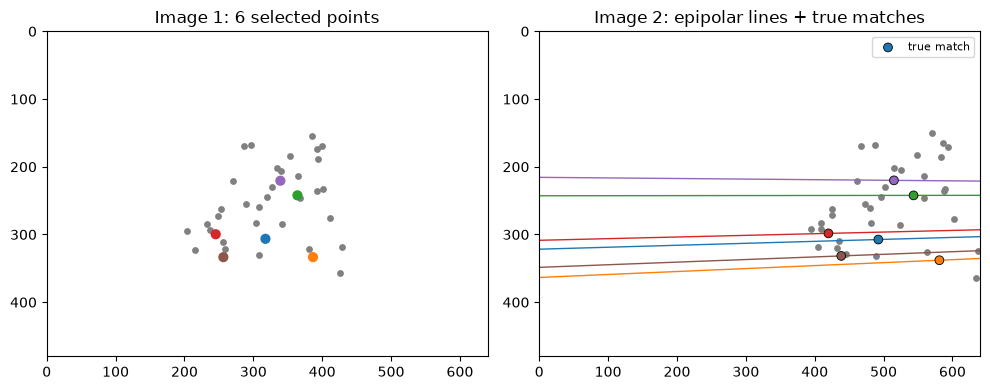
\includegraphics[width=0.95\textwidth]{figures/lesson28_fig03.png}
\caption{6 selected points in image 1, and their predicted epipolar lines $l_2=Fx_1$ in image 2 --- every true match lands exactly on its predicted line, confirming a point's search in the second image really does collapse from 2D to 1D, even without rectifying the images first.}
\label{fig:l28-3}
\end{figure}

\section{From fundamental to essential: adding calibration}

The fundamental matrix works in raw pixel coordinates, assuming the camera intrinsics are unknown. If the intrinsics $K$ are known (from calibration, Chapter~\ref{ch:lesson27}), the intrinsics can be removed, giving the \textbf{essential matrix}:
\begin{equation}
E = K_2^\top F K_1 \qquad \text{(same camera: } K_1=K_2=K\text{)}.
\end{equation}
Unlike $F$'s 7 degrees of freedom, $E$ has only 5 --- it's built entirely from a relative rotation $R$ and translation direction $t$: $E=[t]_\times R$, where $[t]_\times$ is the skew-symmetric cross-product matrix of $t$. This means $E$ can be \emph{decomposed} back into $R$ and $t$, which is how camera motion is recovered from image correspondences alone. Estimating $E$ robustly with \code{cv2.findEssentialMat(..., method=cv2.RANSAC, ...)} --- the same outlier-rejecting fit built from scratch in Chapter~\ref{ch:lesson23} --- agrees with $E$ derived directly from $F$ and $K$ to 4 decimal places.

\subsection*{Recovering camera motion}

\code{cv2.recoverPose} decomposes $E$ into a rotation and a translation \emph{direction} --- not a full translation vector, since the magnitude is fundamentally unrecoverable from two views alone (a scene twice as large, viewed by cameras with twice the baseline, produces identical images --- the same scale ambiguity familiar from monocular vision). On the synthetic scene: the recovered rotation matches the true $15^\circ$ rotation to 3 decimal places, and the recovered translation direction matches the true direction up to the expected sign convention.

From feature correspondences alone (Chapter~\ref{ch:lesson20}), we've recovered the relative rotation and translation (up to scale) between the two cameras --- the starting point for structure from motion (Chapter~\ref{ch:lesson29}).

\subsection*{Exercises}
\begin{enumerate}
  \item Add pixel noise (e.g.\ std $0.5$) to the correspondences before running the 8-point algorithm. How much does the mean epipolar residual grow, and does normalizing coordinates actually matter here --- try skipping the normalization step and compare.
  \item The epipole in image 2 is the projection of camera 1's center, and satisfies $Fe_1=0$ for the epipole $e_1$ in image 1 (and $F^\top e_2=0$ for the epipole $e_2$ in image 2). Compute both epipoles as the null space of $F$ (via SVD) and check whether they fall inside or outside the visible image region for this camera configuration.
  \item Increase the rotation angle between the two cameras to $60^\circ$ and rerun pose recovery. Does \code{cv2.recoverPose} still find the correct rotation? At what point would you expect correspondence matching itself (Chapter~\ref{ch:lesson20}) to become the bottleneck rather than the geometry?
\end{enumerate}

\vfill
\fullcode{lesson28}{lesson28_epipolar_geometry}
